%%%%%%%%%%%%%%%%%%%%%%%%%%%%%%%%%%%%%%%%%%%%%%%%%%%%%%%%%%%%%%%%%%%%%%%%%%%%%%%%
%2345678901234567890123456789012345678901234567890123456789012345678901234567890
%        1         2         3         4         5         6         7         8
% THESIS CHAPTER

\chapter{System architecture and hardware/software used}
\label{chap:third}
\ifpdf
    \graphicspath{{Chapter3/Figures/PNG/}{Chapter3/Figures/PDF/}{Chapter3/Figures/}}
\else
    \graphicspath{{Chapter3/Figures/EPS/}{Chapter3/Figures/}}
\fi


% short summary of the chapter
\section*{Summary}
% Discuss here the methodology used in the study, the stages by which the methodology was implemented, and the research design; For examples, one section details the participants in the study, another section lists all the instruments used in the study and justifies their use; another section outlines the procedure (algorithms, code,..) used; a section discusses how the data was analysed, etc..
In this chapter the design of our system is explained to give an
idea of how the idea of this project is applied to the TTN architecture.
In the other section we describe the devices and software used in order
to achieve the objective.

\section{Proposed system model}
\label{sec:s-system}
The next figure describes the proposed system in a graphical way to make it clear:
\begin{figure}[htbp]
    \includegraphics[width=\linewidth]{System.png}
    \caption{Proposed system}
\end{figure}

This LoRaWan system that is implemented starts with the laptop running the Arduino 
program on the adafruit board. The LoRaWan communication module of the board
is capable of transmitting LoRaWan packets to the gateway. This comunnication is the one 
in which the measurements will be taken, so is the one that will be analized in this thesis. 
The gateway is connected to the Internet via the operator networkand the data sent by the gateway 
will arrive first to the network server of TTN and then to our respective application server. 
The laptop is also making HTTP requests in order to analize the data from the database of the 
application server using python, specifically the library matplotlib. This architecture allows 
to analize the LoRaWan communication, which is the goal of this project.

\section{Devices used and their implementation}

\subsection{The gateway} 
\label{sec:s-gate}
The model of gateway used for this is the indoor Dragino lps-8. This device is forwarding LoRaWan 
packets via internet. This gateway acts like a bridge connecting the LoRaWan wireless network 
with the Internet. The indoor model was selected because in this case the gateway is fixed inside 
a building.
The gateway is on the 5$^{th}$ floor, connected to wall 
power through a USB-C port near a window in order to have the best possible . The access to the internet is 
provided through WiFi connection to the house router/modem. The configuration of the router was done 
as it is ilustrated in the figure \ref{chap:third:fig:gwconf}:

\begin{figure}[htbp]
    \includegraphics[width=\linewidth]{GatewayConfig.png}
    \caption{Configuration of the gateway via WiFi}
    \label{chap:third:fig:gwconf}
\end{figure}

On google maps, with a scale of 20 meters as shown in the image at figure \ref{sec:s-gw:loc}

The gateaway was located in the pinpoint shown in figure \ref{sec:s-gw:loc} 
\begin{figure}[htbp]
    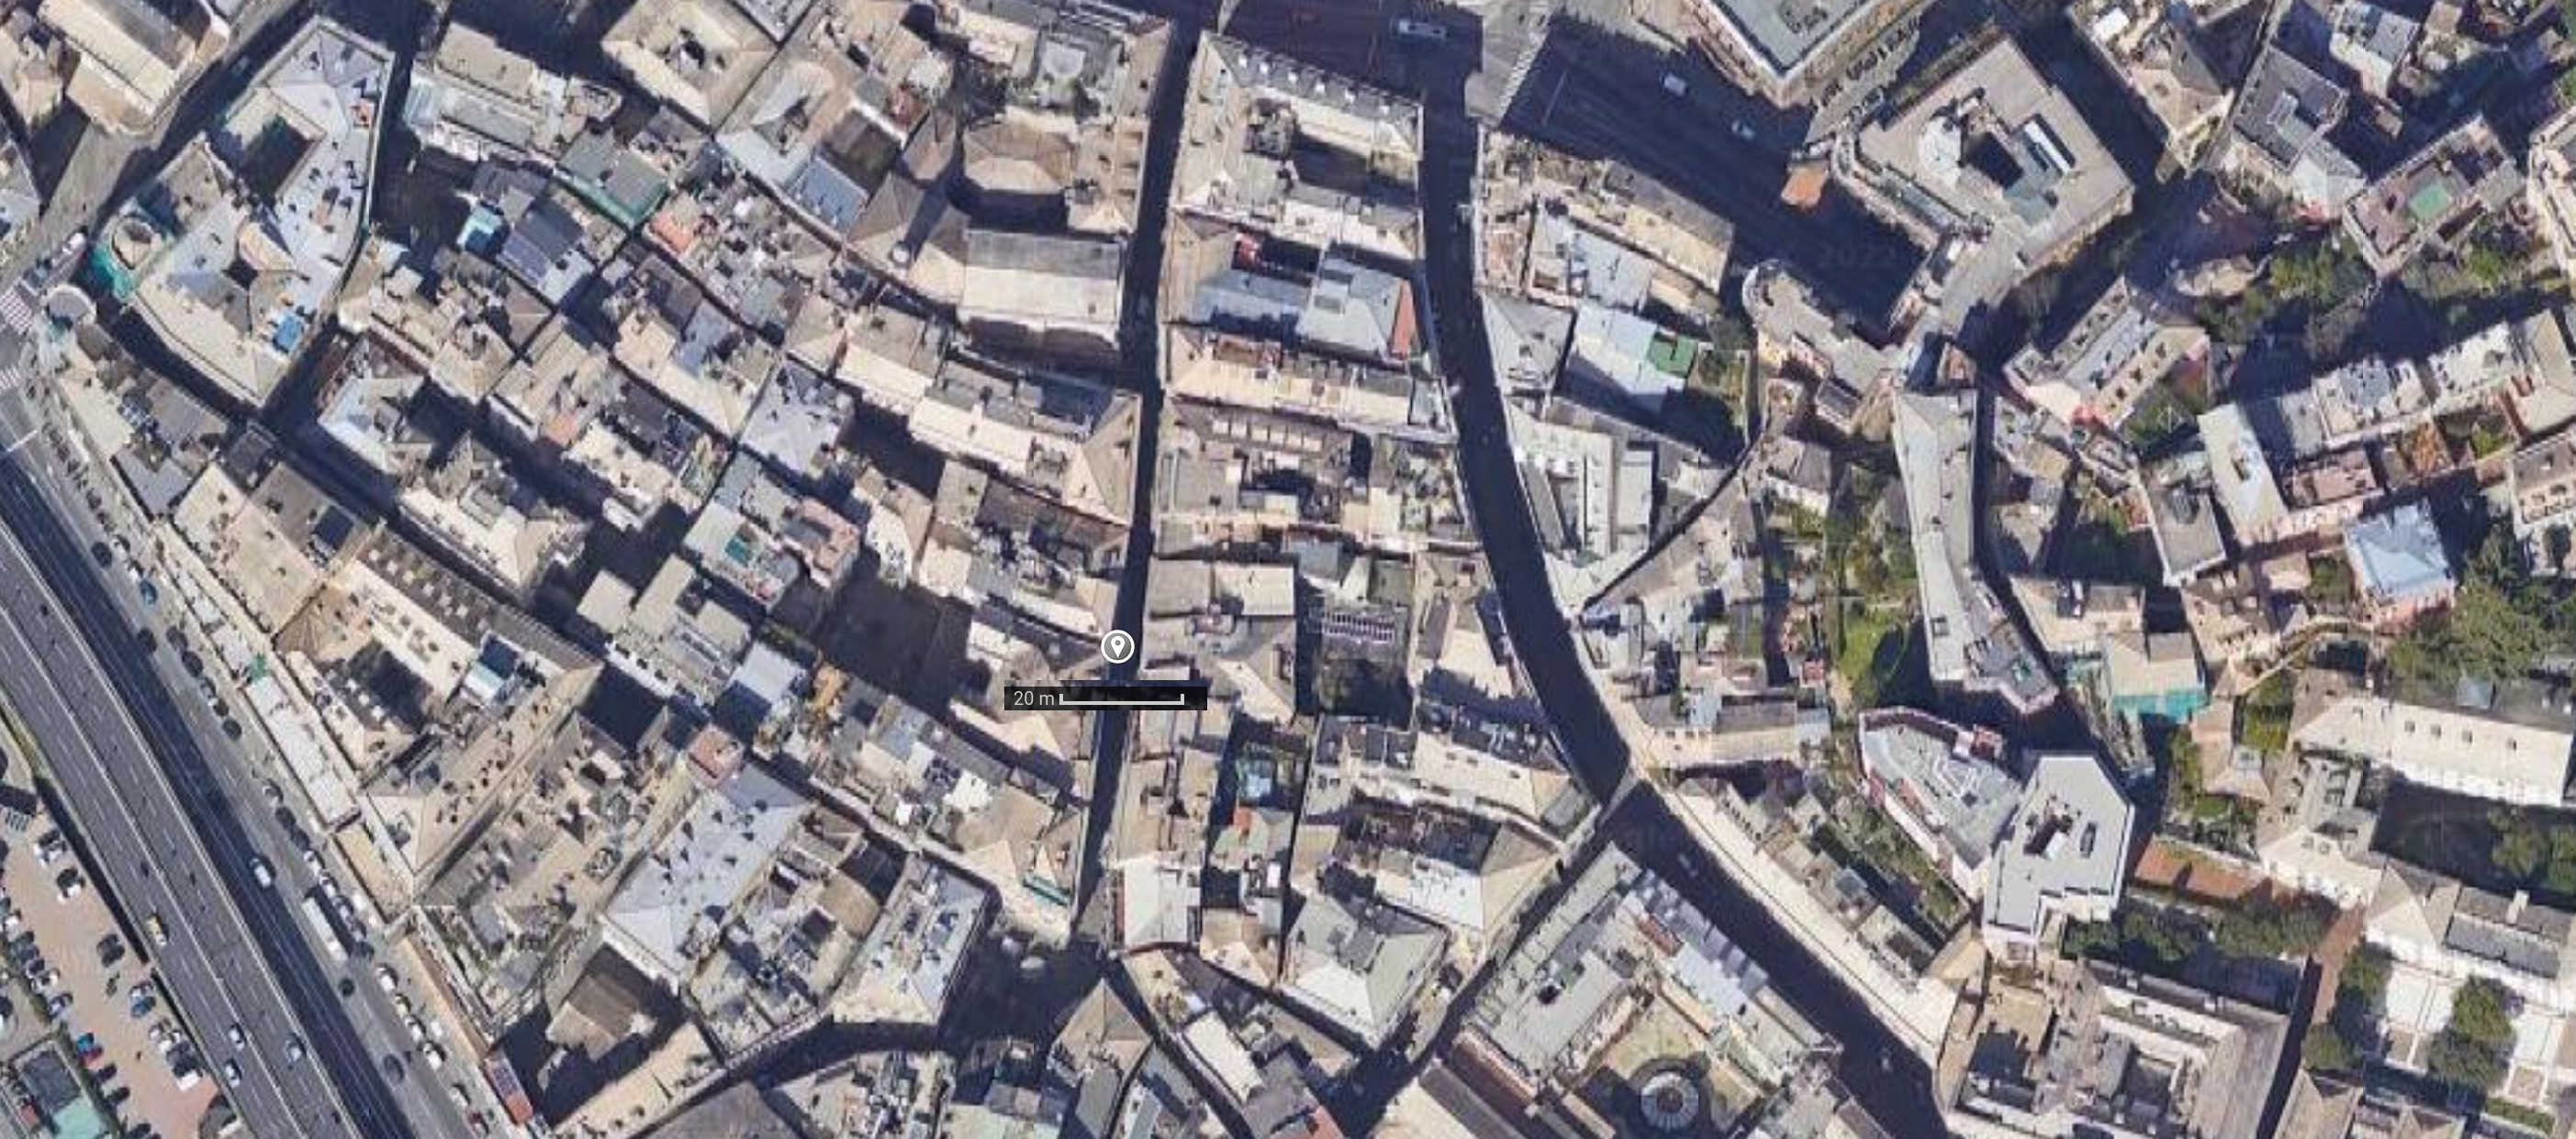
\includegraphics[width=\linewidth]{mapaloragateway.png}
    \caption{Location of the gateway on the map}
    \label{sec:s-gw:loc}
\end{figure}


\section{The microcontroller}
\label{sec:s-micro}
The microcontroller used as a node in the network is the Adafruit Feather
M0 RFM95 LoRa Radio. The device is equipped with a transceptor
module LoRa, with built in USB and battery charging. The processor is
a ATSAMD21G18 ARM Cortex M0 at 48MHz and 3.3v (the same as the
Arduino Zero) and a quarter of a megabyte of FLASH, with 32k of RAM.
Thanks to the USB port, and a bootloader, the device can be
programmed and debugged through the USB port, no need for an
external programmer, which would have been yet another thin layer of
complexity.\\ 
\begin{figure}[htbp]
\includegraphics[width=\paperwidth, angle = 90]{pinout.png}
\caption{The pinout of the module}
\end{figure}
More info of the board and the pinout can be found \href{https://learn.adafruit.com/adafruit-feather-m0-radio-with-lora-radio-module/pinouts}{here}
The I2S connectors were used to connect the sensors which
communicated through the protocol, and DIO1 was manually wired to
GPIO6 so that the radio would work. For each individual sensor a different connection may be needed, so in
general, we connected the I2S to the same pins SCI and SDA and the
simple voltage for temperature sensor was connected directly to the
GPIO A0, setting it to an input on software to read from it.

\subsection{Sensors}
The first sensors mentioned were used to introduce us to the Arduino and IoT enviroment and the last one (the gps module)
is the one we finally used in order to measure the distance between the node and the gateway:
\begin{itemize}
    \item[-] Temperature and humidity sensors: 
        \begin{itemize}
        \item The \href{https://www.ti.com/lit/ds/symlink/hdc1080.pdf?ts=1655758883138&ref_url=https%253A%252F%252Fwww.google.com%252F}{hdc1080 sensor}
        is a digital humidity sensor with integrated temperature sensor that provide respective measurents using low power consumption.
        \item Another sensor with similar purpose is the \href{https://cdn-learn.adafruit.com/downloads/pdf/adafruit-bme280-humidity-barometric-pressure-temperature-sensor-breakout.pdf}{bme280 sensor}.
        in addition to the other one this sensor is capable of measuring preassure appart of temperature and humidity. 
        \end{itemize} 
        Two of this sensors were used and the respective models are hdc1080 bme280
    \item[-] Air quality sensor: sensor of the brand \code{SPEC SENSORS} specifically the model
    \href{https://www.spec-sensors.com/wp-content/uploads/2016/10/ULPSM-IAQ-968-008.pdf}{ULPSM-IAQ}. 
    It measures the indoor air quality   with very low power consumption and the output signal in this case is analog.

\end{itemize} 
This sensors are designed for the IoT enviroment as all of them use low power consumption. This characteristic is optimal 
for the purpose of LoRaWan networks using the less power consumption as possible. 

\subsection{GPS module and antenna}
The module \href{https://www.u-blox.com/en/product/lea-6-series}{u-block LEA-6S-0-001} 
is able to obtain the specific coordinates in which the module is placed with a precission of 2.5m and 
it's also designed for low power consumption. \\

This module is designed for the use of passive and active antenna. The antenna selected for this gps module is an 
active one, which means that the received signal is amplified. The available freaquency bands are the following ones:

\begin{figure}
    \includegraphics[width = \linewidth]{GPS_frequency_bands.png}
    \caption{Center frecuency and BW for the three different GPS bands}
\end{figure}

In our case we will work with 1575 MHz as it is the band that detects our antenna.



\section{Software used}
\label{sec:s-m-soft}

\subsection{MCCI LMIC Arduino library}
\label{sec:s-m-lmic}

The \code{MCCI\_LoRaWAN\_LMIC} library was the most complete library for
our purpose. The recommended library by Adafruit has the flaw of not
being compliant with the TTN standard anymore as it cannot receive
downlink messages, and the RadioHead library is a LoRa library,
requiring us to implement the whole LoRaWAN engine for ourselves.
\code{MCCI\_LoRaWAN\_LMIC} library is already done so there was no need to
waste our efforts. For more information about the library, the
documentation, code and repository are 
\href{https://github.com/mcci-catena/arduino-lmic.}{here}. The library is a pretty big and complex piece of C code, so a brief
explanation will be given.
Using the 4.1.0 version, so it will be the model explained:
(GPS Click - Breakout Board for u-blox LEA-6s, 2022)

\begin{figure}[htbp]
\centering
\includegraphics[width=\paperwidth, angle= 90]{modelLMIC.png}
\caption{Finite state machine of LMIC library}
\label{sec:lib-finitestate}
\end{figure}
In figure \ref{sec:lib-finitestate} is pictured the whole finite state machine. The only part a user should be
concerned about is the frame data set up, the actions to be taken for
every event desired to react to with the \code{onEvent()} call-back function
or \code{LMIC\_registerEventCb()} API function. Both are currently
supported, and although the \code{onEvent()} application call-back is
currently deprecated, it still works on version 4 and it is simple to
implement and debug. The other option is the recommended one, but is
harder to comprehend.
We ended with a function that, when the package is sent, a timed call-
back is issued thanks to the convenience function
\code{os\_setTimedCallback()} to schedule a job in the next
\code{TX\_INTERVAL}, that job in charge of queuing up another packet of data
to be sent, witch will be collected by the engine and, when sent, the cycle
starts once again: \\
first job → sent → wait TX → job → sent → wait TX → job ... \\
This is “interrupted” by the compliance engine, that ensures that
the law is not broken by keeping track of the air time so that the device
can't send more than the percentage set by the region configuration in the library
(currently on EU 868).
The I2C library was used to communicate with the sensors, as a
dependency of the particular libraries for each one of them.
\code{ClosedCube\_HDC1080} library was used for the more straightforward
and the \code{Adafruit\_BME280} was used for the other sensor.

\subsection{TinyGPSPlus}
\label{sec:s-m-tinygps}
This library is design to parse all type of NMEA data that the GPS module provides. In our case this 
library is used in order to extract the exact latitude and longitude of the ED. More info about this 
library can be found in the \href{https://github.com/mikalhart/TinyGPSPlus}{github repository}

\subsection{U-center}
\label{sec:s-m-ucenter}
The software developed by the company u-block is a monitoring system for the gps module mentioned before. 
U-center provides info about the signal that gps is detecting from the gps-satellites. Once the gps is 
calibrated the u-center software provides all data the gps is collecting including the longtude and latitude.

\subsection{Arduino}
\label{sec:s-m-lmic}

\subsection{Python}
\